\documentclass{chi-ext}

% some more configurations
%-- Package hyperref ------------------------------------------------------------------------------
\usepackage[
	plainpages=false, %Gibt an auf welcher Seite die pdf-Darstellung beginnt.
	pdfpagelabels,
	pdftex=true,
	breaklinks=true, %/false: Gibt an, ob Links umgebrochen werden duerfen.
	%linktocpage=true/false: im Inhaltsverzeichnis sind nur die Seitenzahlen links, nicht der Text
	colorlinks=true, %/false: Links werden eingefaerbt (Farben werden mit linkcolor, anchorcolor ... festgelegt)
	linkcolor=black, %Farbe des verlinkten Textes, Dokument-interne Links
	citecolor=black, %Farbe des verlinkten Textes, Links zum Literaturverzeichnis
	filecolor=black, %Farbe des verlinkten Textes, Links auf lokale Dateien
	urlcolor=black, %Farbe des verlinkten Textes, externe URLs
	%frenchlinks=true/false: Links werden als smallcaps, anstatt farbig dargestellt.
	menucolor=black
]{hyperref}

\hypersetup{
	pdftitle={GreenSubway},
	pdfauthor={Andreas Jahn, Stephan Sigg},
	pdfsubject={GreenSubway},
	pdfkeywords={GreenSubway},
	%pdfpagelayout={TwoColumnRight}
	%bookmarksnumbered=true,
	%bookmarksopen=true,
	%bookmarksopenlevel=1,
	%pdfpagemode=None % None, UseOutline, UseThumbs, FullScreen
}
\usepackage{balance}  % to better equalize the last page

\usepackage{graphicx}   % for EPS use the graphics package instead
% \usepackage{balance}    % useful for balancing the last columns
\usepackage{bibspacing} % save vertical space in references
\usepackage{rotating}
% \usepackage{multirow}
% \usepackage{subfig}

\begin{document}

\title{\plaintitle}


\numberofauthors{4} %  in this sample file, there are a *total*
% of EIGHT authors. SIX appear on the 'first-page' (for formatting
% reasons) and the remaining two appear in the \additionalauthors section.
%
\author{
% You can go ahead and credit any number of authors here,
% e.g. one 'row of three' or two rows (consisting of one row of three
% and a second row of one, two or three).
%
% The command \alignauthor (no curly braces needed) should
% precede each author name, affiliation/snail-mail address and
% e-mail address. Additionally, tag each line of
% affiliation/address with \affaddr, and tag the e-mail address with \email.
%
% 1st. author
\alignauthor{
	\textbf{Andreas Jahn}\\
	\affaddr{Kassel University}\\
	\affaddr{Wilhelmh\"oher Allee 73}\\
	\affaddr{Kassel, Germany}\\
	\email{andreas.jahn@uni-kassel.de}
	}\alignauthor{
	\textbf{Klaus David}\\
	\affaddr{Kassel University}\\
	\affaddr{Wilhelmh\"oher Allee 73}\\
	\affaddr{Kassel, Germany}\\
	\email{david@uni-kassel.de}
	}
\vfil
\alignauthor{
	\textbf{Stephan Sigg}\\
	\affaddr{Goettingen University}\\
	\affaddr{Goldschmidtstr. 7}\\
	\affaddr{G\"ottingen, Germany}\\
	\email{stephan.sigg@informatik.uni-goettingen.de}
    }\alignauthor{
	\textbf{Xiaoming Fu}\\
	\affaddr{Goettingen University}\\
	\affaddr{Goldschmidtstr. 7}\\
	\affaddr{G\"ottingen, Germany}\\
	\email{fu@informatik.uni-goettingen.de}
    }
}

% Title
\maketitle

% Abstract
\begin{abstract}
CCTV camera systems for monitoring and surveillance are widely utilised in enterprises or public systems. 
They can provide a holistic view on a system and allow security and maintenance personnel to quickly react on changes in the system in an informed manner.
However, mostly, the analysis of the data is done manually which is a tedious task and prone to errors or the missing out of information. 
Automatic analysis of such video-recorded data can help to improve this task in efficiency and accuracy and also enables novel applications build on top of it. 

In this paper we present the work done in the SEAM4US consortium that focuses on the automatic analysis of image data captured from CCTV cameras in a Barcelona metro system and to react on the extracted stimuli. 
We present the sensing environment and detail specifics of the system, introduce the steps for feature extraction from the video data, discuss peculiarities of the recorded data and demonstrate its predictability with an Adaptive Network-based Fuzzy Inference System (ANFIS).
\end{abstract}

% Author Keywords - Mandatory section to be included in your final version.
\keywords{\plainkeywords}%config.tex

% ACM Classification Keywords - Mandatory section to be included in your final version.
%\category{H.5.m}{Information interfaces and presentation (e.g., HCI)}{Miscellaneous}. 
%See: \url{http://www.acm.org/about/class/1998/} for help using the ACM Classification system.

% General Terms - optional NOT mandatory
%\terms{\plaingeneralterms}


% Introduction
\section{Introduction}
\label{sec:introduction}

Underground transportation systems are big energy consumers and have significant impacts on energy consumptions at a regional scale~\cite{anderson_maximizing_2009}. 

So far the optimization of the energy efficiency of transportation equipments, e.g. trains have been considered. Optimization of the energy efficiency of the metro stations operations, however, is only minimally exploited.

But realizing savings in energy consumption are meaningful for two reasons:
(\textit{i})~Despite the relatively small percentage that can be gained with optimal management of one metro station compared to optimizing trains, the high numbers of metro stations in the underground transportation will yield large energy savings in overall terms. In other words, in the management of metro stations is a high multiplication factor that boosts each relative small saving at a station level to a high saving at a metro network level.
Moreover (\textit{ii}) the optimization of the energy efficiency of the metro stations involves much less investments than the ones that are usually applied to transportation means and equipments. Consequently is it possible to distributed the technology easily across the whole metro network, as well as other transportation systems and realize savings in short term.

For example all Barcelona (Spain) metro stations consumes 63,1 millions of kWh annually~\cite{TMB}. A relative small saving of, e.g. 5\% in the electricity consumption of one metro station, is equivalent to the electricity consumed in more than 700 households during one year.

The optimized management of stations and surroundings, such as ventilation, vertical transportation and lighting does have an impact.

An approach to optimize the energy efficiency and to realize energy savings is to
enable the station to control the surroundings, such as ventilation, vertical transportation and lighting "intelligent" according the current situation. 
A simple example of "intelligent" control could be the slowing down the frequency of the ventilation-fans of the station, when the count of passenger doesn't make full speed necessary.

To achieve the context aware behaviour of a metro station basically two parts are necessary. (i) A controller which calculate the appropriate actions. A controller which is adaptive on the basis of various environmental factors, forecasts and passenger occupancy was developed~\cite{guo_intelligent_2013}.
(ii) The environmental factors, and prediction must be available for the controller. 

Staying in the given example the controller needs be aware about the current count of passengers in order to decrease the fan frequency if possible. However, increasing the fan frequency is more complex. Since the decreasing of the fan frequency doesn't have an immediate effect for the air quality the fan frequency needs to be decreased in a appropriate time before the stations is abruptly crowed again. To guarantee the required air quality on every point in time, the ventilation needs to be controlled in a foreseen manner, i.e. controlled on the prospectively number of passenger in the station.

This paper presents an approach for predicting the prediction of number of passenger in the station.

The remainder of this paper is organized as follows. In Section~\ref{sec:stateOfTheArt} an overview of the related literature is given. Section~\ref{sec:dataAcquisition} focuses on the data acquisition and the experiments, followed by Section~\ref{sec:results}, the evaluation and results. Last, Section~\ref{sec:conclusion}, summarizes the results.


% SEAM4US & pilot station & CCTV
\section{Environment}
\label{sec:environment}

Underground transportation systems have significant impacts on energy consumption at a regional scale. While the transportation systems, i.e. trains, has observed regarding energy efficiency, the subsystems of metro stations and surroundings, such as ventilation, escalator and lightning are mostly unexplored.

Although a nominally small percentage of energy can be saved with an efficient management of these subsystems, a large energy saving in absolute terms can be obtained. In other words a 5\% energy saving in non-traction electricity consumption in one year, is equivalent to the electricity consumed in more than 700 households. 

\subsection{SEAM4US project}
\label{subsec:seam4us}

To research in the area of energy efficient surroundings, the EU funded the "Sustainable Energy mAnageMent for Underground Stations"~(SEAM4US) project in the Seventh Framework Programme.
The aim of SEAM4US project "is to develop advanced technologies for optimal and scalable control of metro stations [...]. The project's main outcomes will be the creation of systems for optimized integrated energy management, and the development of a decision support system to drive mid-term investments"~\cite{SEAM4US_Website}.
The integrated energy management is realized by employing passenger density models and thermal models, integrating sensors and control algorithms in a model predictive control architecture~\cite{ansuini_models_2013}. The control architecture proactively controls the metro station surroundings (ventilation, escalator, and lightning) under different occupancy and thermal conditions.

The SEAM4US consortium consists of nine partners from six different EU countries, namely Cofely, UniVPM, UPC, Fraunhofer FIT, VTT, Almende, University of Kassel, CNET and TMB.

Cofely is a major player in energy-efficient system management sector.
UniVPM and UPC are experts in building and environmental physics and construction.
Fraunhofer~FIT and VTT support the consortium as R+D experts in middleware.
Almende and UniKassel research in area of user and agent-based scheduling modeling and CNet supports as system integrator.
The large metro network operator Transports Metropolitans de Barcelona~(TMB) supports with its experience with underground systems as well as the model underground station.
A overview over the SEAM4US consortium is given in Table~\ref{tab:SEAM4USconsotium}.

\begin{table}[htbp]
  \centering
  
    \begin{tabularx}{\columnwidth}{|X|c|}
	\hline
    \textbf{Name} & \textbf{Country} \\
	\hline
    Cofely Italia Spa & Italy \\
	\hline
    Universita Politecnica Delle Marche & Italy \\
	\hline
    Universitat Politecnica De Catalunya & Spain \\
	\hline
    Fraunhofer-Gesellschaft Zur Foerderung Der Angewandten Forschung E.V & Germany \\
	\hline
    Teknologian Tutkimuskeskus VTT & Finland \\
	\hline
    Universitaet Kassel & Germany \\
	\hline
    Almende B.V. & Netherlands \\
    	\hline
    CNet Svenska AB & Sweden \\
    	\hline
    	Ferrocarril Metropolita De Barcelona Sa & Spain \\
	\hline
    \end{tabularx}%
    
  \caption{SEAM4US consortium}%
  \label{tab:SEAM4USconsotium}%
\end{table}%


\subsection{Metro Station "Passeig de Gr\`{a}cia"}
\label{subsec:station}

%TODO http://www.tmb.cat/en/detall-linia-metro/-/linia/L3/327

%TODO
The implementation of the developed technologies is done in one of the stations of the partner TMB in Barcelona.
To validate the system, it is installed in a underground station in Barcelona.
This section describes the "station" in detail, while the word "station" in the area of metro networks needs to be defined first.

Starting high level, a metro network is composed by one or more metro lines. Each line has a fixed railway with a given number of stops to allow people to get on or off the trains by means of a platform: each of these stops is called "line station". A "metro station" is the concept that represents the point in space through which a passenger gets underground and into a line station. Metro station and line station can be the same physical entity, but it is possible that there are some "metro stations" that receive two or more "metro lines" in different platforms, and have therefore, two or more "line stations" within.

The data, used in this work, are gathered in line station in Passeig de Gr\`{a}cia - Line~3~(PdG-L3) located in Barcelona. Passeig de Gr\`{a}cia~(PdG) is a station in the metro network of "Transports Metropolitans de Barcelona"~(TMB) and lies in a very iconic and touristic part of Barcelona. Some of the popular buildings designed by Antoni Gaud\'{i} are in the proximity (Casa Batll\`{o}, Casa Mil\`{a}), as well as the city's most renown and exclusive boutiques.
The metro station is one of the oldest of the Barcelona metro network. First opened in December of 1924, as a (line) station for Line~3, nowadays PdG holds three different line stations: L2, L3, and L4. The stations were built in three different periods and using different construction technologies. All line stations has been refurbished a few times since 1924 and new equipment has been added recently.

\begin{figure}[htb]
  \centering
  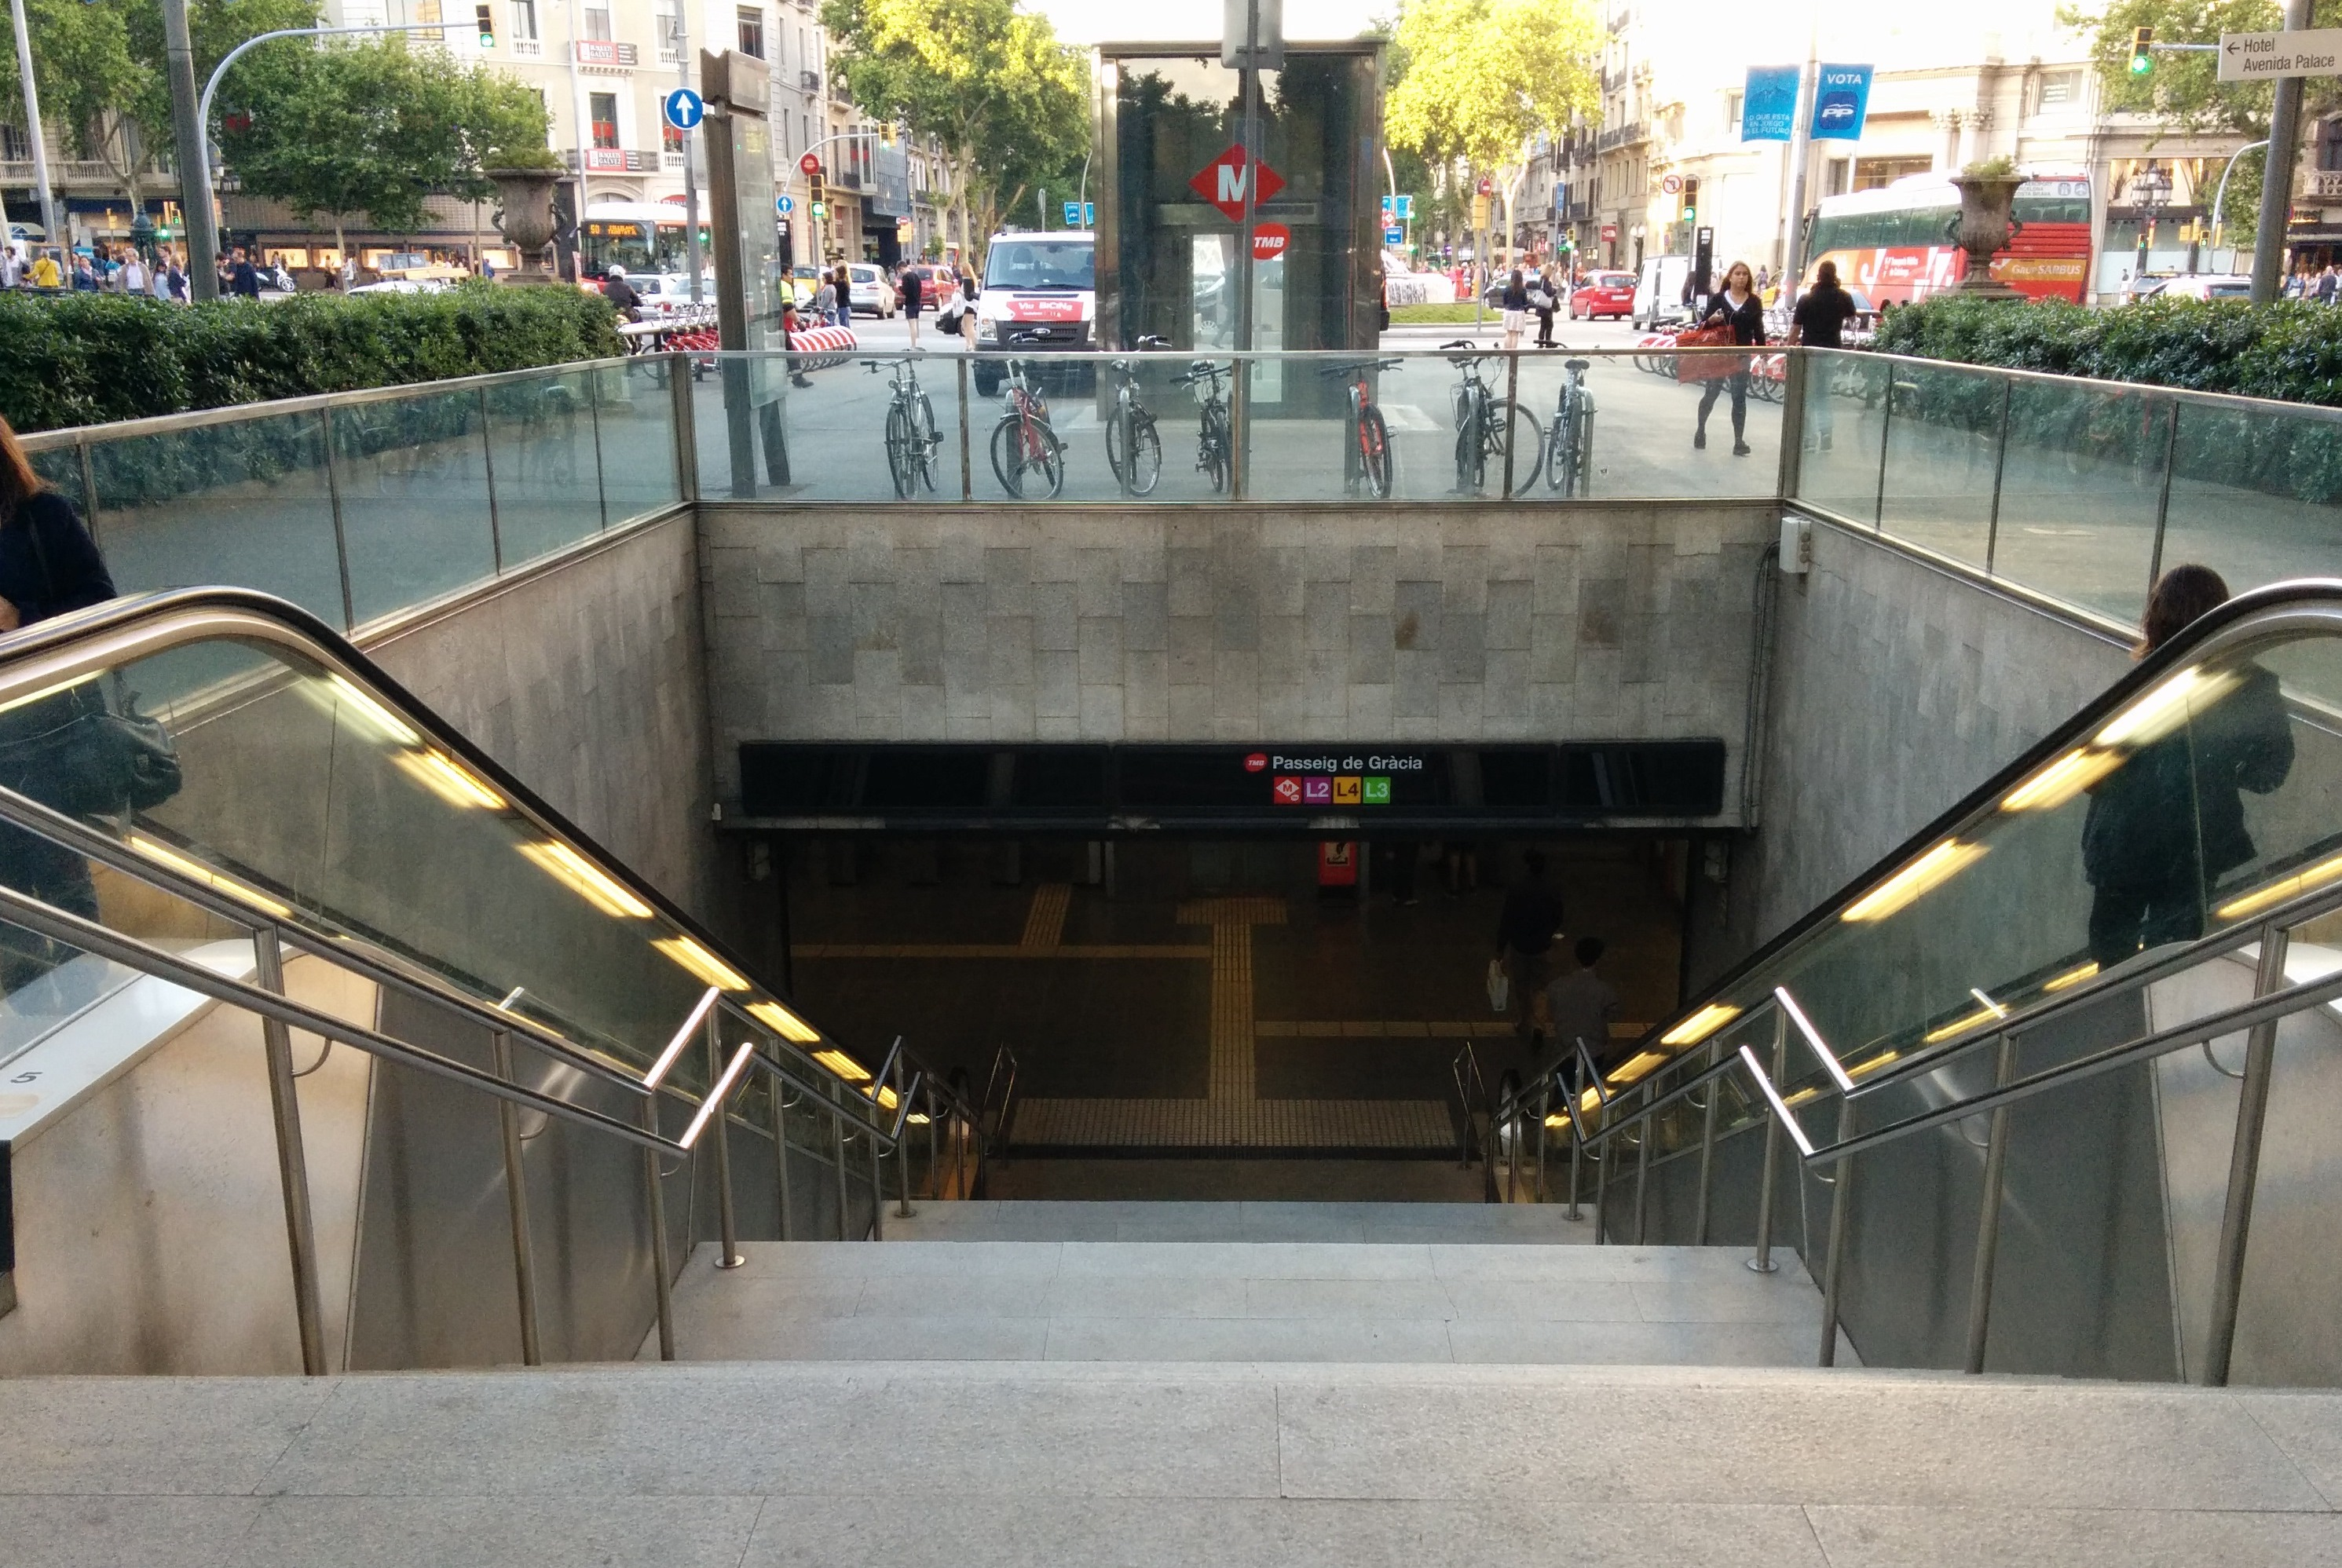
\includegraphics[width=\linewidth]{Figures/PdG-L3_entranceExit.jpg} 
  \caption{PdG Entrance/Exit Gran Via. \cite{TMB_2014}}
  \label{fig:PdG_entranceExit}
\end{figure}

Depending on the weekday PdG is open 19~hours, 21~hours or 24~hours. Between Monday and Thursday PdG service starts at 5:00 and ends at 24:00 (19~hours). Friday service starts at 5:00 and ends at 2:00 (21~hours). On Saturday service starts at 5:00 to but remain the entire night until midnight on Sunday.

Passeig~de~Gr\`{a}cia - Line~3~(PdG-L3) turns out to be representative for many station within TMBs metro network~\cite{TMB}. Moreover PdG-L3 is a crowded station which have low-rate usage hours as well. This provides a wide range of data which allows to test with very busy peak hours as well as with off-peaks.

The line station PdG-L3 consists of private (staff only) and public spaces. Private spaces such as technical rooms or staff dependencies are not part of the investigation. Public spaces, such as halls, transit areas, accesses to the platforms, and platforms are however in the focus on the SEAM4US project.

Essential part of underground line stations are the platforms, which allow passengers to leave and enter trains. PdG-L3 laid out on a PRRP (Platform-Rail-Rail-Platform) schema. The platforms in PdG-L3 are visible on Figure~\ref{fig:PdG-L3_platforms}.

\begin{figure}[htb]
  \centering
  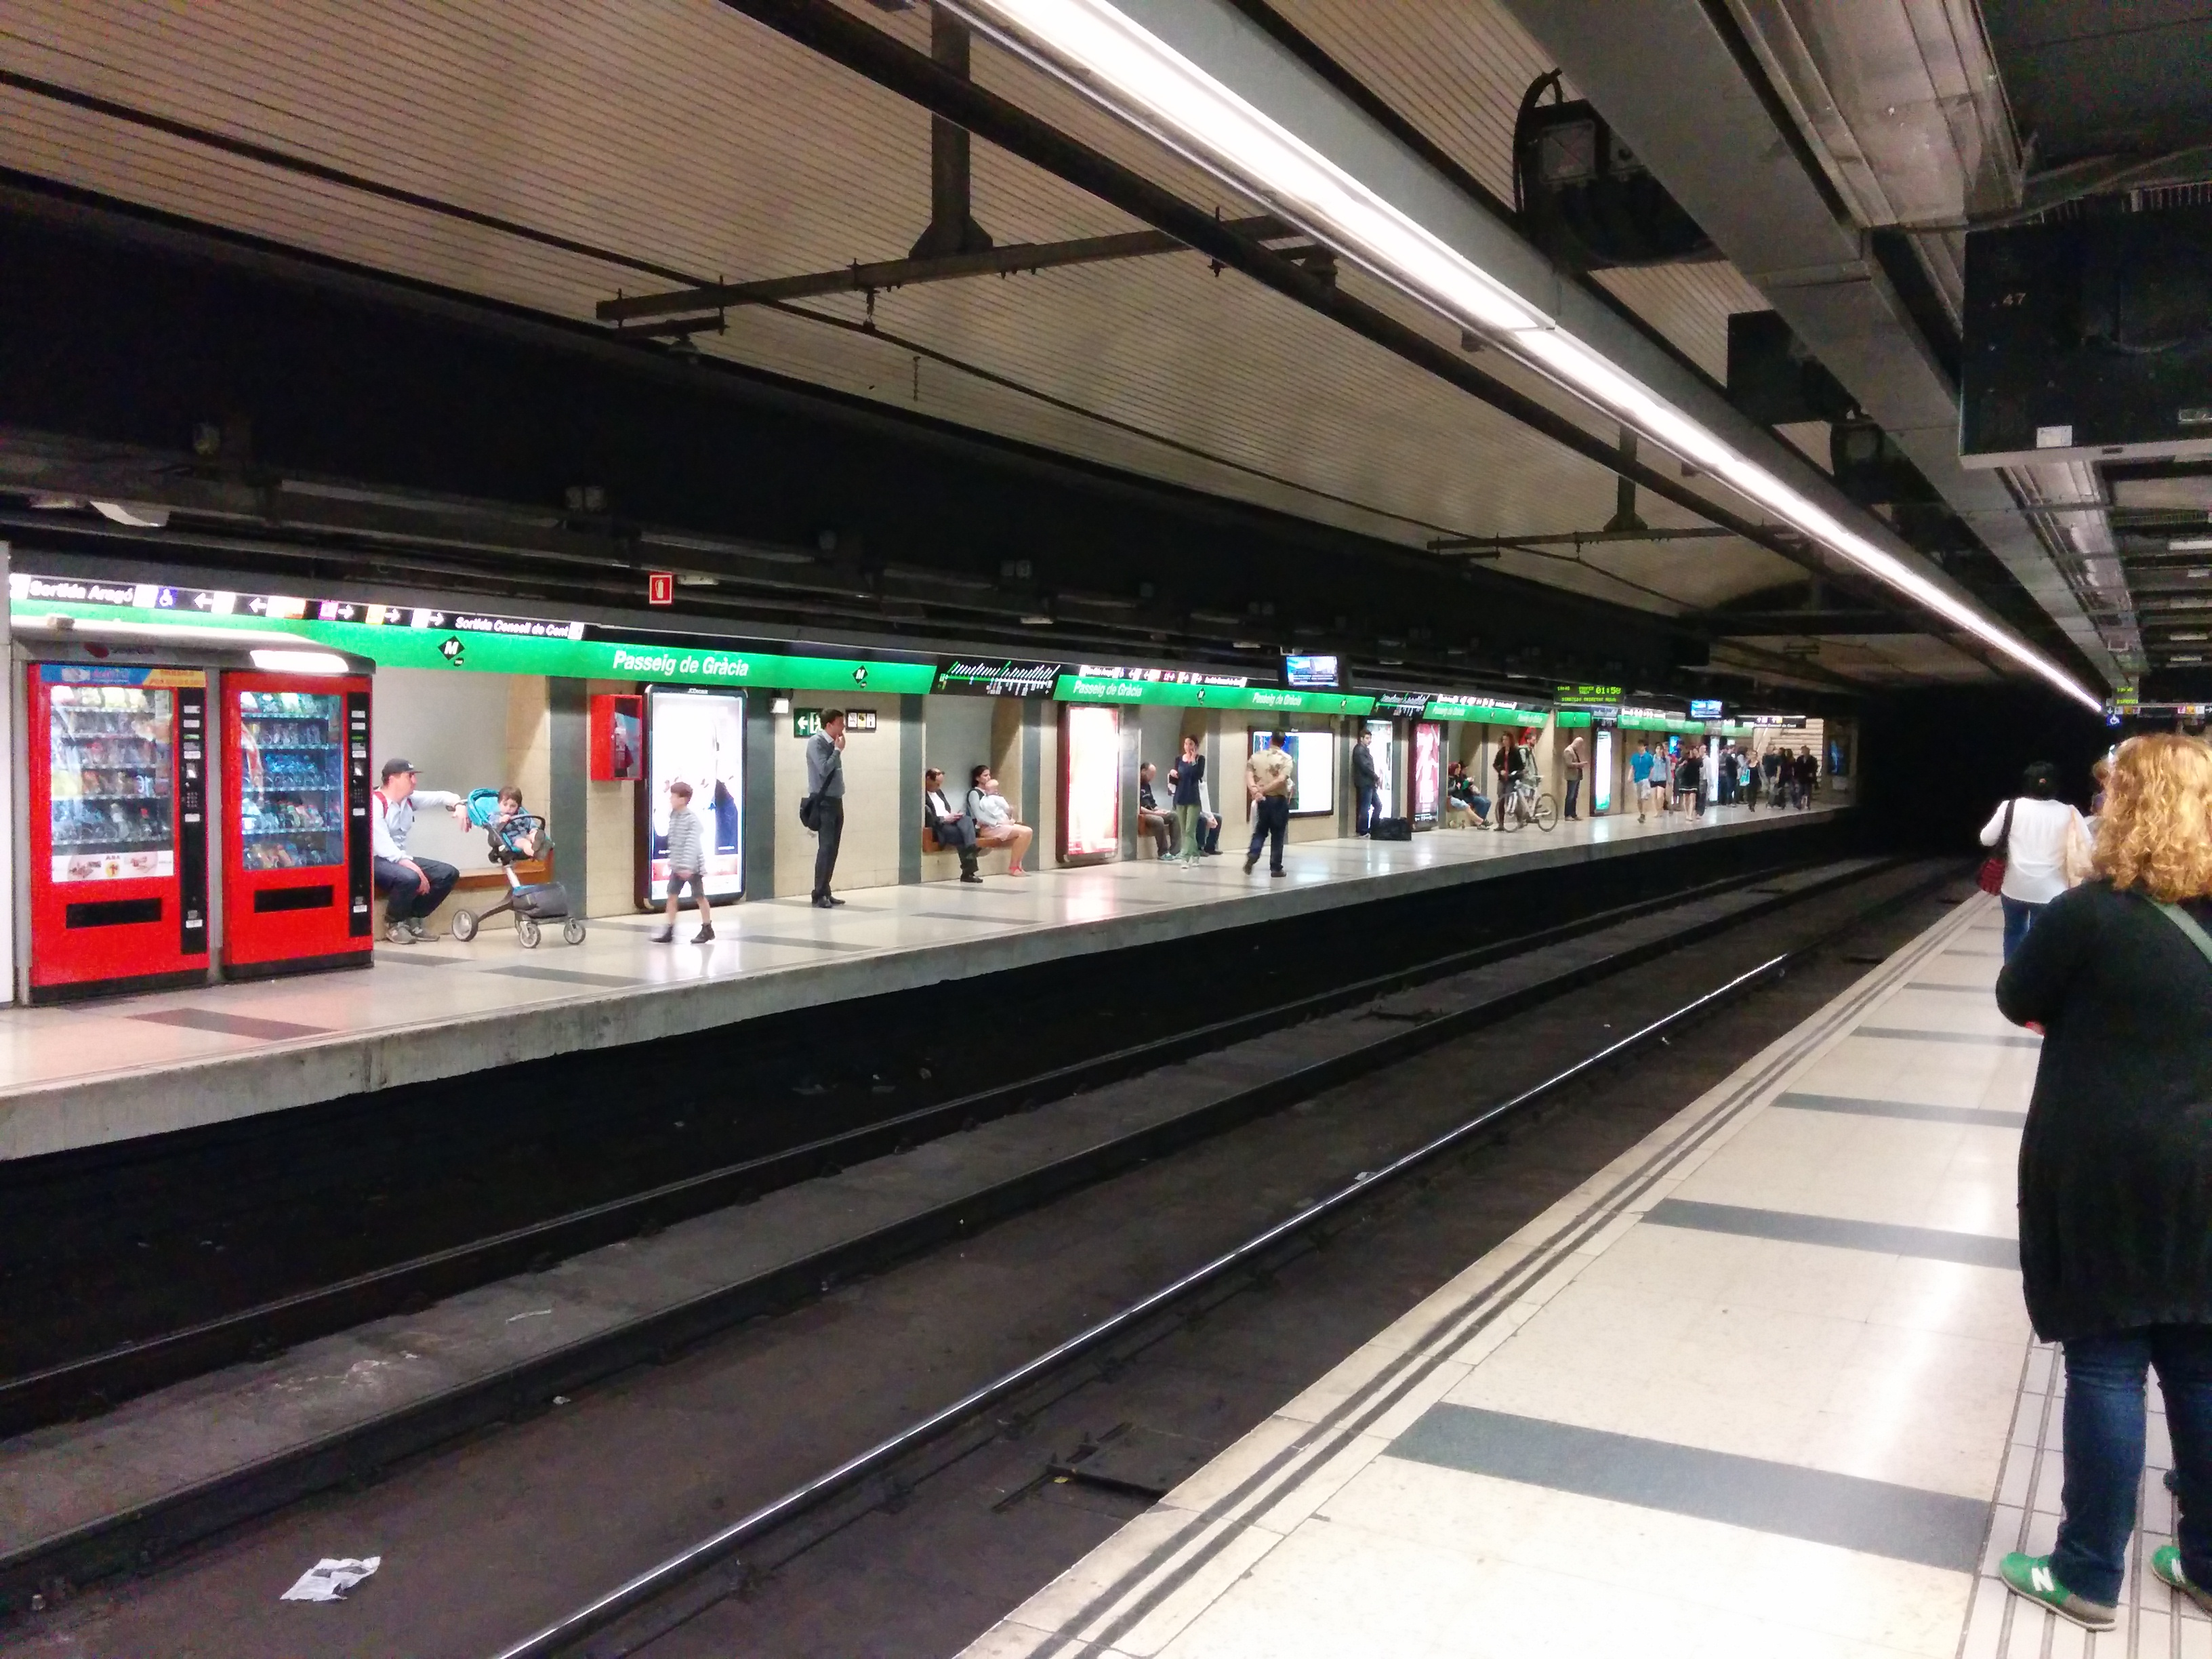
\includegraphics[width=\linewidth]{Figures/PdG-L3_platform.jpg} 
  \caption{PdG-L3 Plattforms. \cite{TMB_2014}}
  \label{fig:PdG-L3_platforms}
\end{figure}


% Escalator image
%\begin{figure}[htb]
%  \centering
%  \includegraphics[width=\linewidth]{Figures/PdG-L3_escalator.jpg} 
%  \caption{PdG-L3 Escalator. \cite{TMB_2014}}
%  \label{fig:PdG-L3_escalator}
%\end{figure}

A schematic representation of PdG-L3 is drawn in Figure~\ref{fig:PdG-L3_schematic}, where the accesses to platforms are highlighted in red.

\begin{figure}[htb]
  \centering
  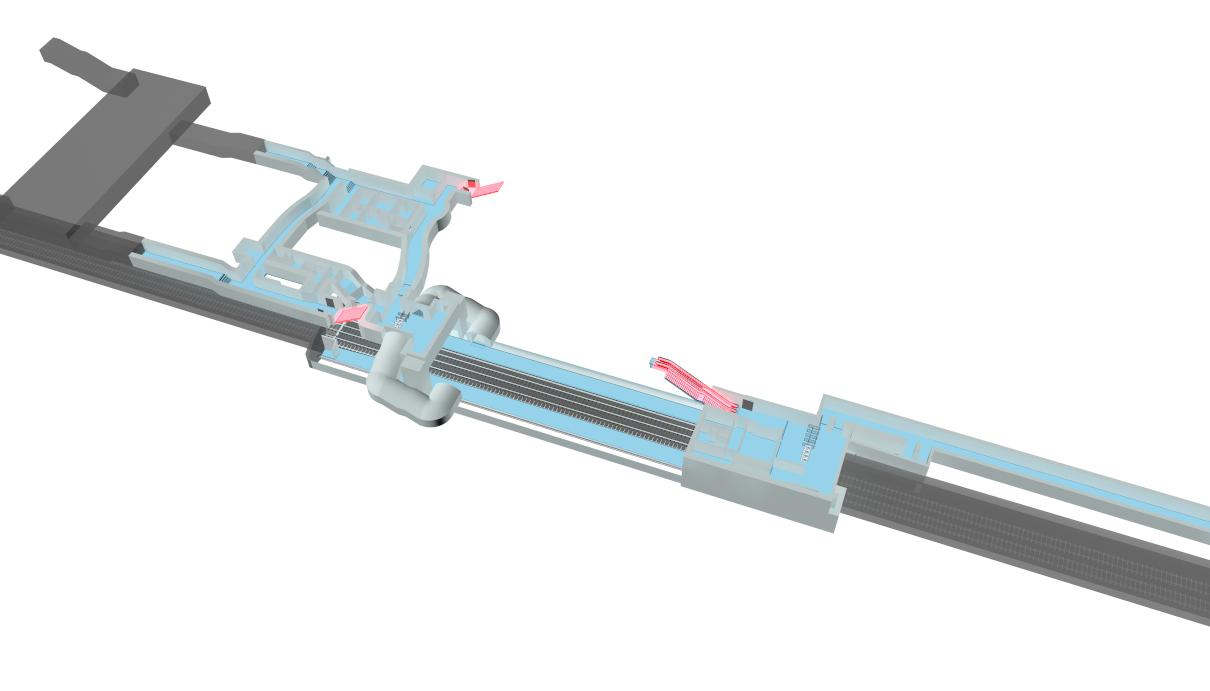
\includegraphics[width=\linewidth]{Figures/PdG-L3_schematic.jpg} 
  \caption{Schematic representation of PdG-L3. The accesses to platforms are highlighted in red. \cite{TMB}}
  \label{fig:PdG-L3_schematic}
\end{figure}

The passenger density models, as one part of the predictive controller, is based on existing CCTV cameras enhanced with image processing to detect current levels of passenger density. In the following section the CCTV~system and the images processing is described briefly.


\subsection{Passenger density level detection}
\label{subsec:PassengerDensityLevelDetection}

Throughout the station a Closed Circuit Television~(CCTV) surveillance system is installed. 20~CCTV~cameras provides images initially for security reasons. Figure~\ref{fig:PdG-L3_CCTVcameras} show exemplary CCTV cameras in a transit area~(Figure~\ref{fig:PdG-L3_CCTVcamera_transitArea}) as well as on the platform~(Figure~\ref{fig:PdG-L3_CCTVcamera_transitArea}).

\begin{figure*}[htb]

  \centering

  \subfigure[CCTV camera installed in a PdG transit area. \cite{TMB_2014}] {
    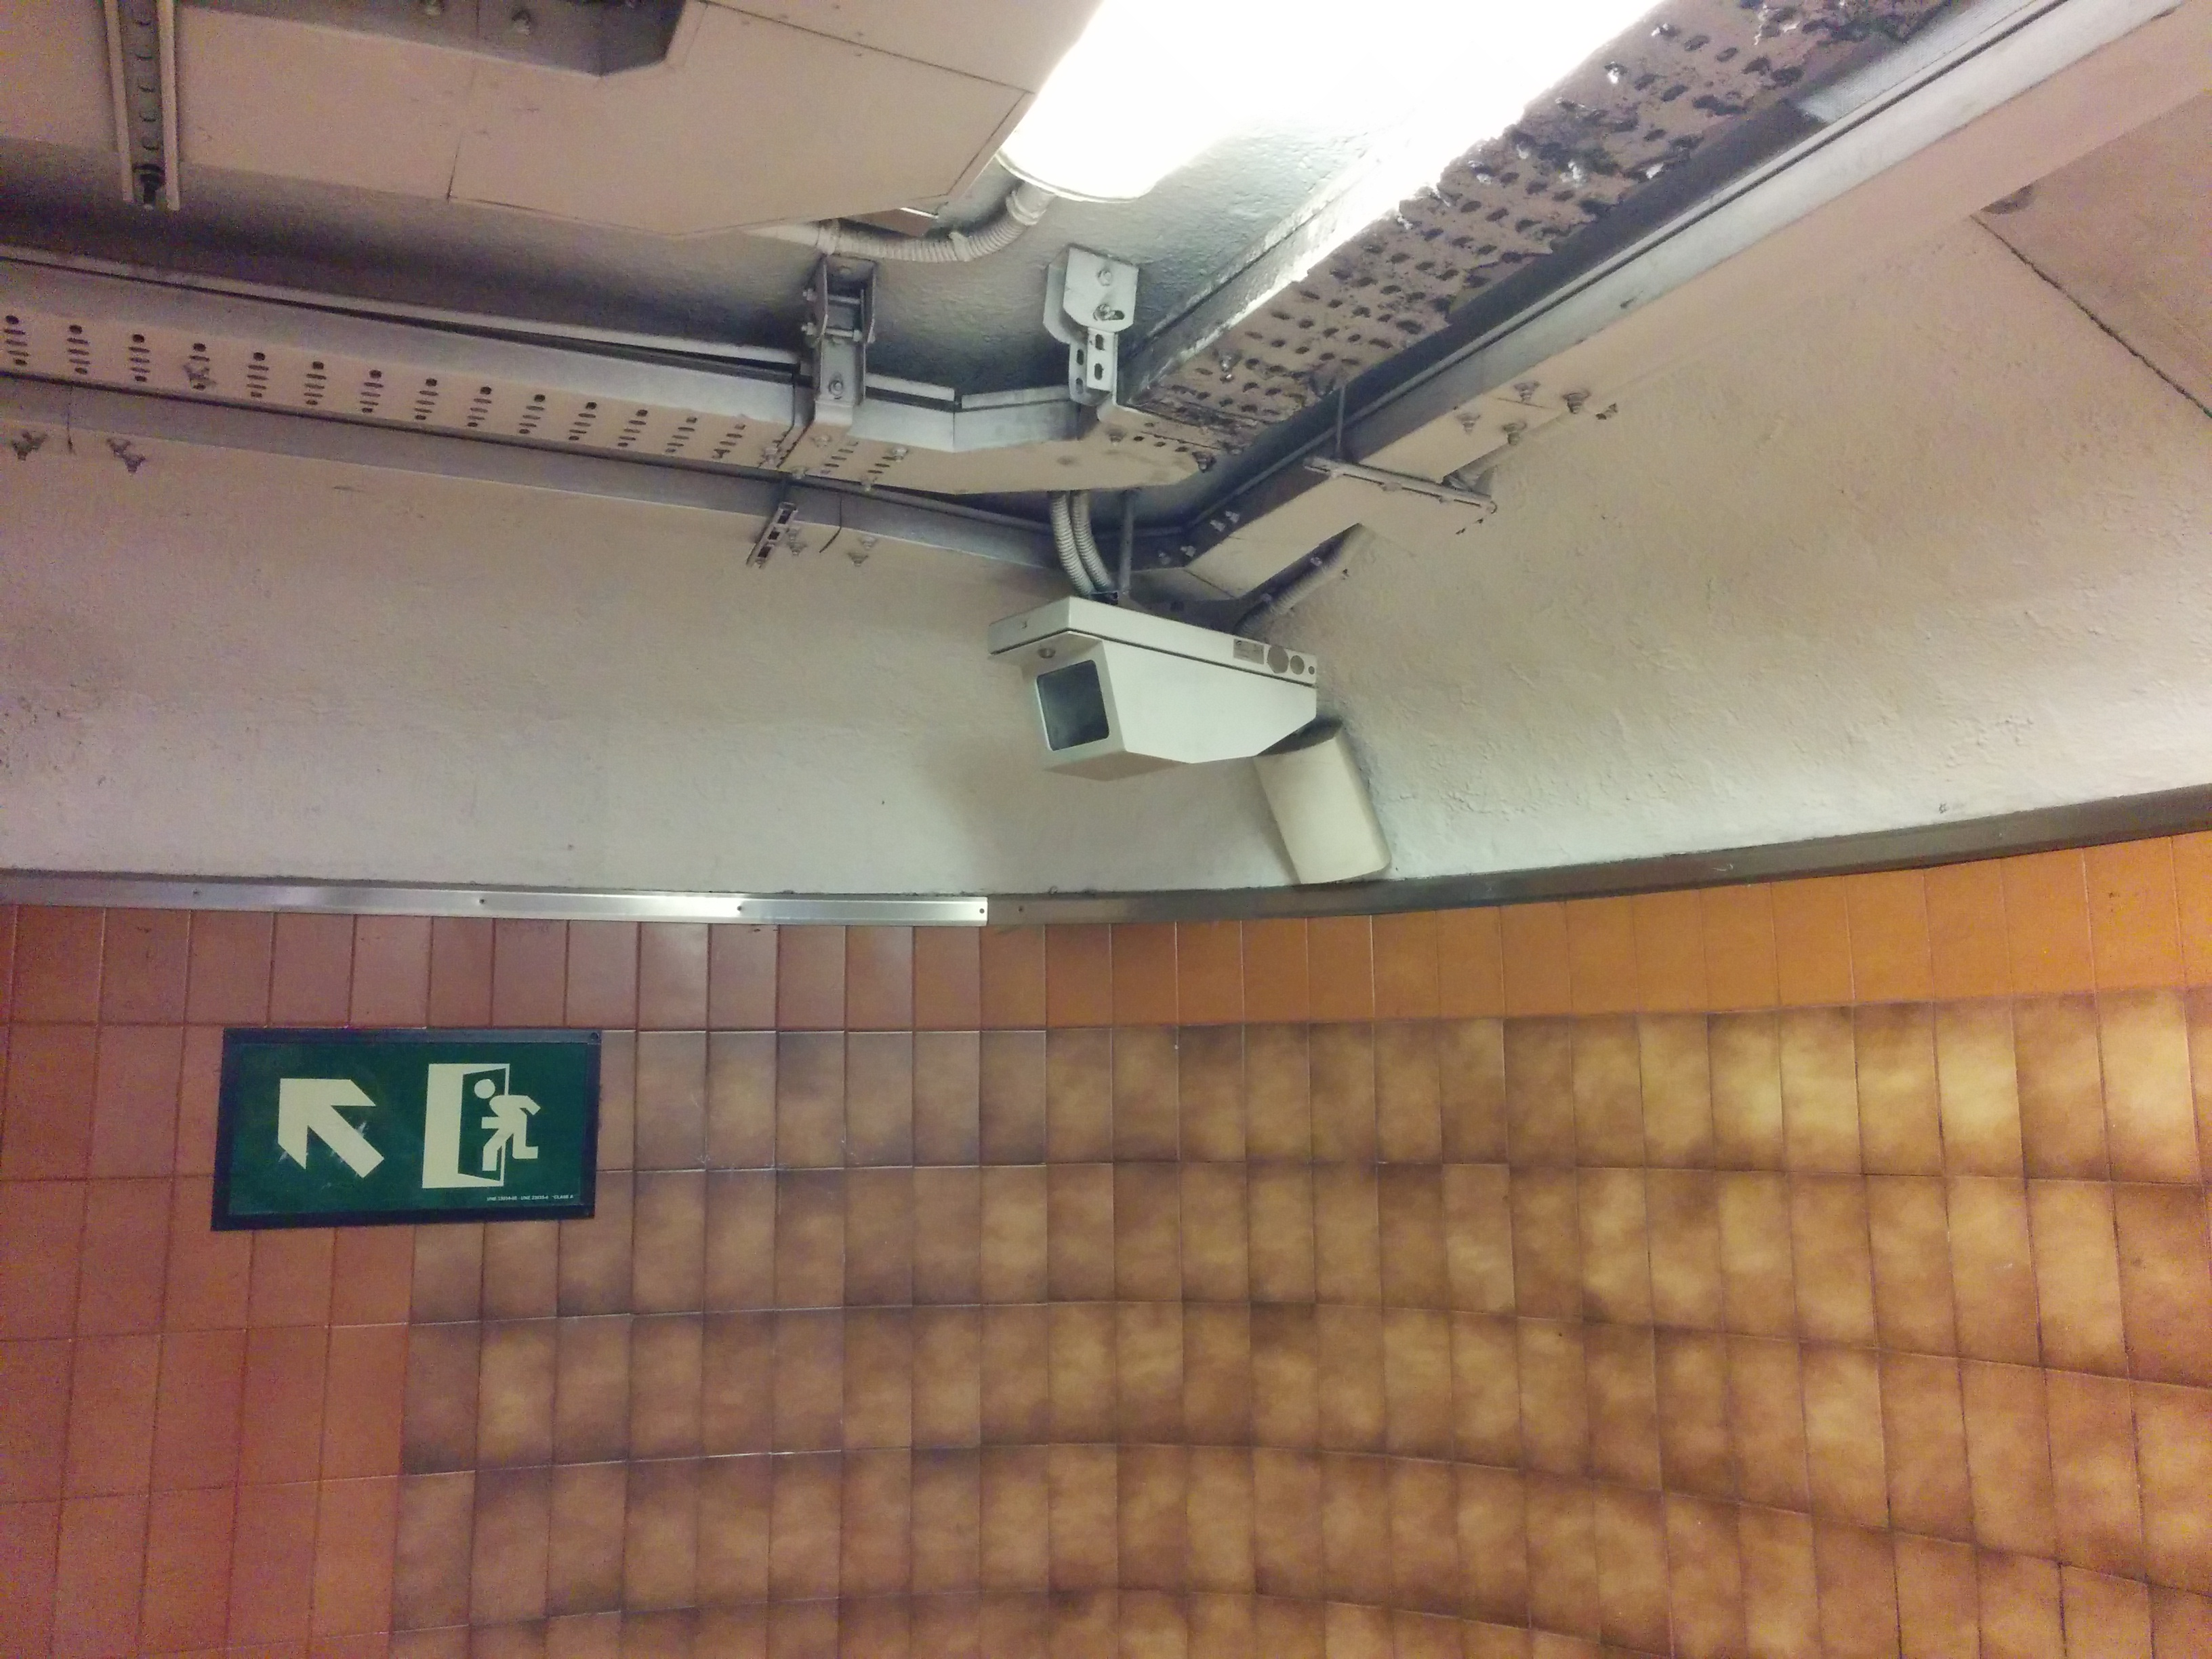
\includegraphics[width=0.46\textwidth]{Figures/PdG-L3_CCTVcamera_transitArea.jpg}
    \label{fig:PdG-L3_CCTVcamera_transitArea}
  }
  \hfill
  \subfigure[CCTV camera installed in PdG-L3 platform. \cite{TMB_2014}] {
    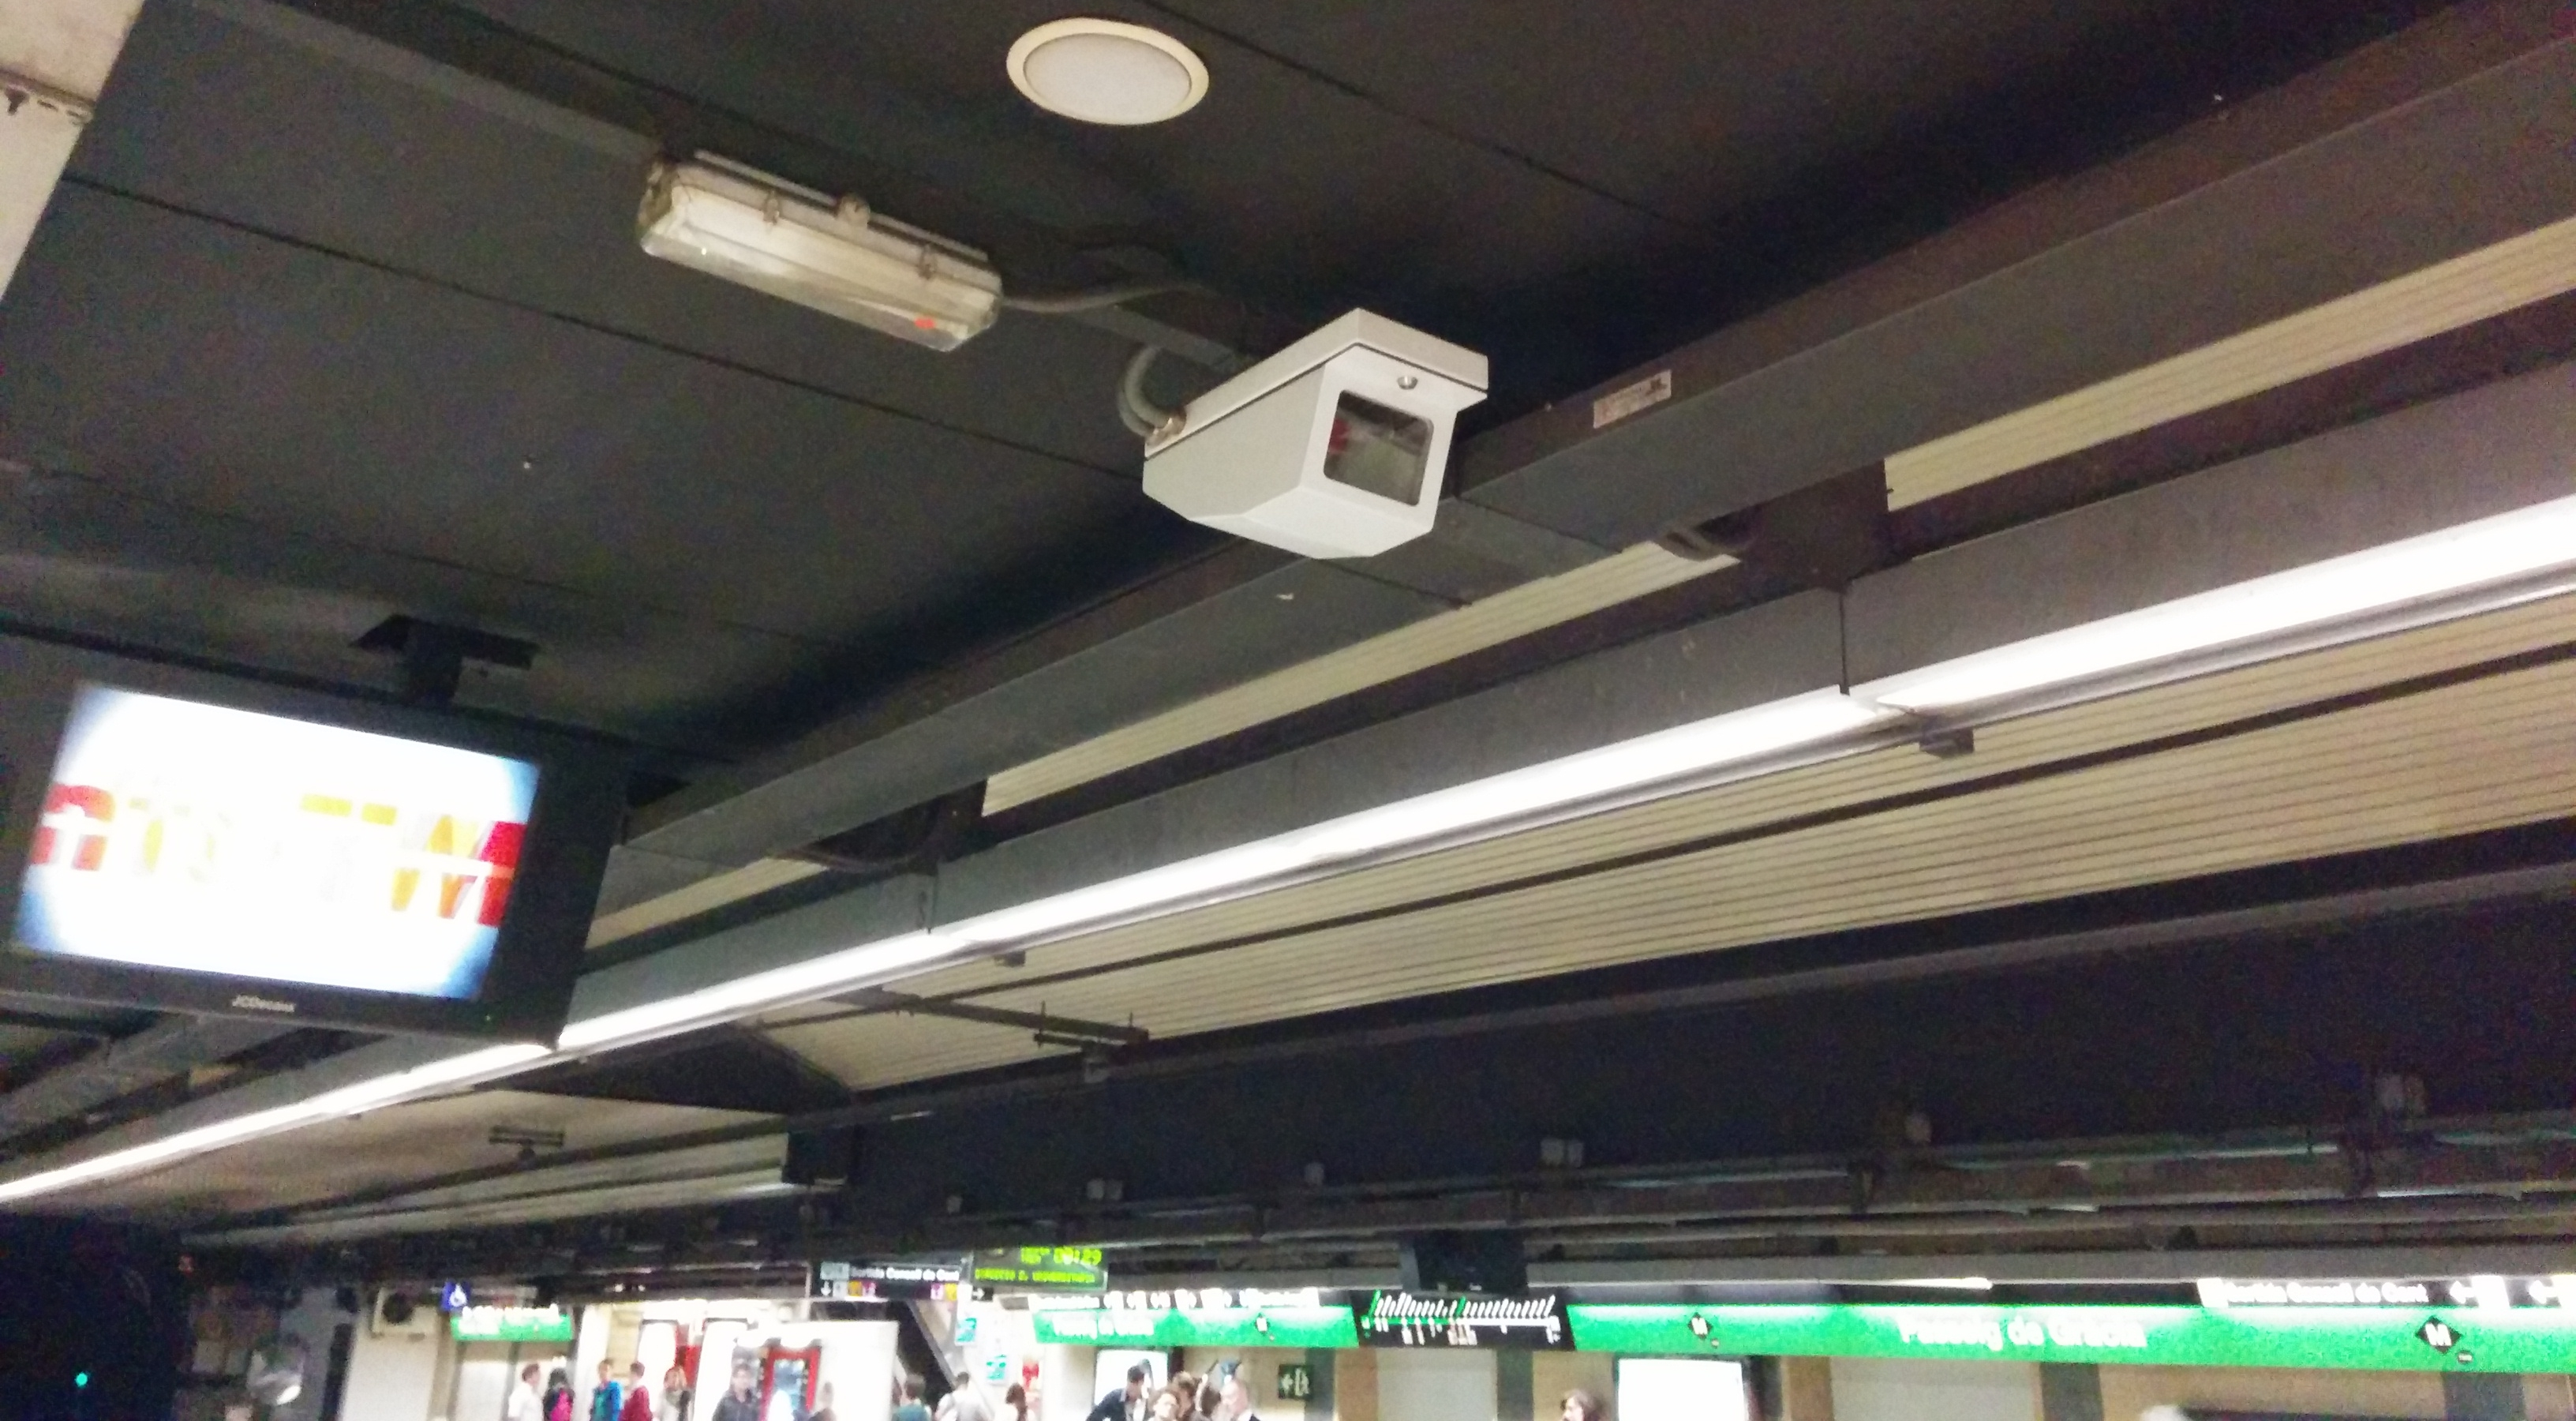
\includegraphics[width=0.46\textwidth]{Figures/PdG-L3_CCTVcamera_platform.jpg}
    \label{fig:PdG-L3_CCTVcamera_platform}
  }

  \caption{Passenger density distribution of one CCTV camera in PdG-L3.}
  \label{fig:PdG-L3_CCTVcameras}

\end{figure*}


The CCTV~system is reused in order to extract the passenger density within the station.

Whenever camera pictures are processed privacy issues are tackled. In order to ensure the passengers privacy several design constrained where defined:
\begin{enumerate}
  \item All CCTV images are processed within the station.
  \item The image processing is performed on a separate computer, which is not connected to other TMB Systems and is only accessible via a dedicated VPN connection.
    \item All CCTV images are processed "on the fly". For the purpose of level of passenger density extraction no CCTV image is saved.
  \item The image processing works without human interaction.
  \item The image data are filtered to avoid recognisability of individuals.
  \item Processing results are transmitting only in terms of integer numbers to the database.
\end{enumerate}

With respect to these design constrains the passenger density extraction was implemented. The work flow is described in the following.

First, the video streams coming from all cameras are combined into one single video stream by a video recorder. This video recorder creates a carousel video composed of sections for the individual camera appearing in a predefined order. The duration of the camera sections is set to 3~seconds. With 20~cameras and 3~seconds hold on each, one turn of the carousel is completed in about one minute.

%The crowd density estimator uses the Real Time Streaming Protocol (RTSP) to establish and control the video recorder.
The video recorder is connected to the local computer and transfer the images subsequently. On the local computer the density estimator processes the transferred images.

%TODO
The crowd density estimator consists of three subcomponents: a) the calibration subcomponent, which sets up several parameters that are needed to make a reliable estimation; b) the computer vision algorithms for crowd density estimation, which is the subcomponent that actually estimates the amount of people focused by each camera; c) the data aggregator, which groups data concerning multiple cameras focused on the same user model zone.
All parts have been developed using the C++ OpenCV libraries.

For different reasons, e.g. occluded or damaged camera, it is possible that the crowd density estimator fails. In this case the image processing return the error value "-1".
The results transmitted to a three~dimensional database, which holds information about the number of passenger, the location and the time.

Finally the passenger density level as well as date, time and the camera-ID of the image are transmitted to the database. The general approach is depicted in Figure~\ref{fig:CCTVimageProcessing}.

\begin{figure}[htb]
  \centering
  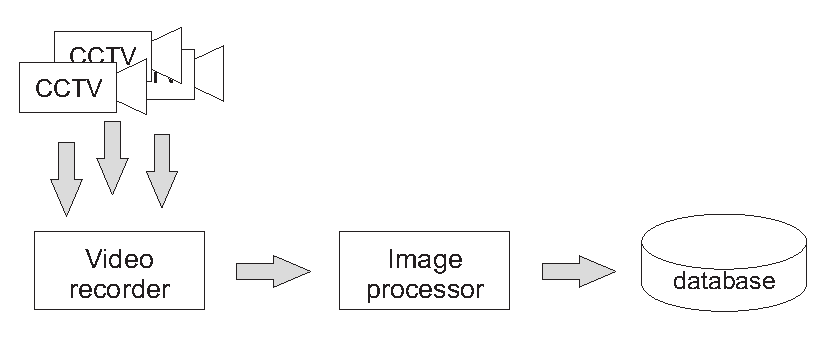
\includegraphics[width=\linewidth]{Figures/imageProcessing.pdf} 
  \caption{Gathering number of people out of the camera images.}
  \label{fig:CCTVimageProcessing}
\end{figure}

The CCTV and image processing runs 24~hours, 7~days a week. Each day 28800~datasets are transmitted to the database. Overall the database contains 90~days of data.

\subsection{Passenger density level}
\label{subsec:PassengerDensityLevel}

Figure~\ref{fig:rawData_week} illustrates exemplary the available values of a camera and week. At a more detailed view Figure~\ref{fig:rawData_day} shows the passenger density level of a camera and (week)day. On both Figures the PdG service times are visible due to the low passenger density level between 1am and 5am on weekdays.

% one column
\begin{figure*}[htb]

  \centering

  \subfigure[Passenger density distribution of one camera during one week.] {
    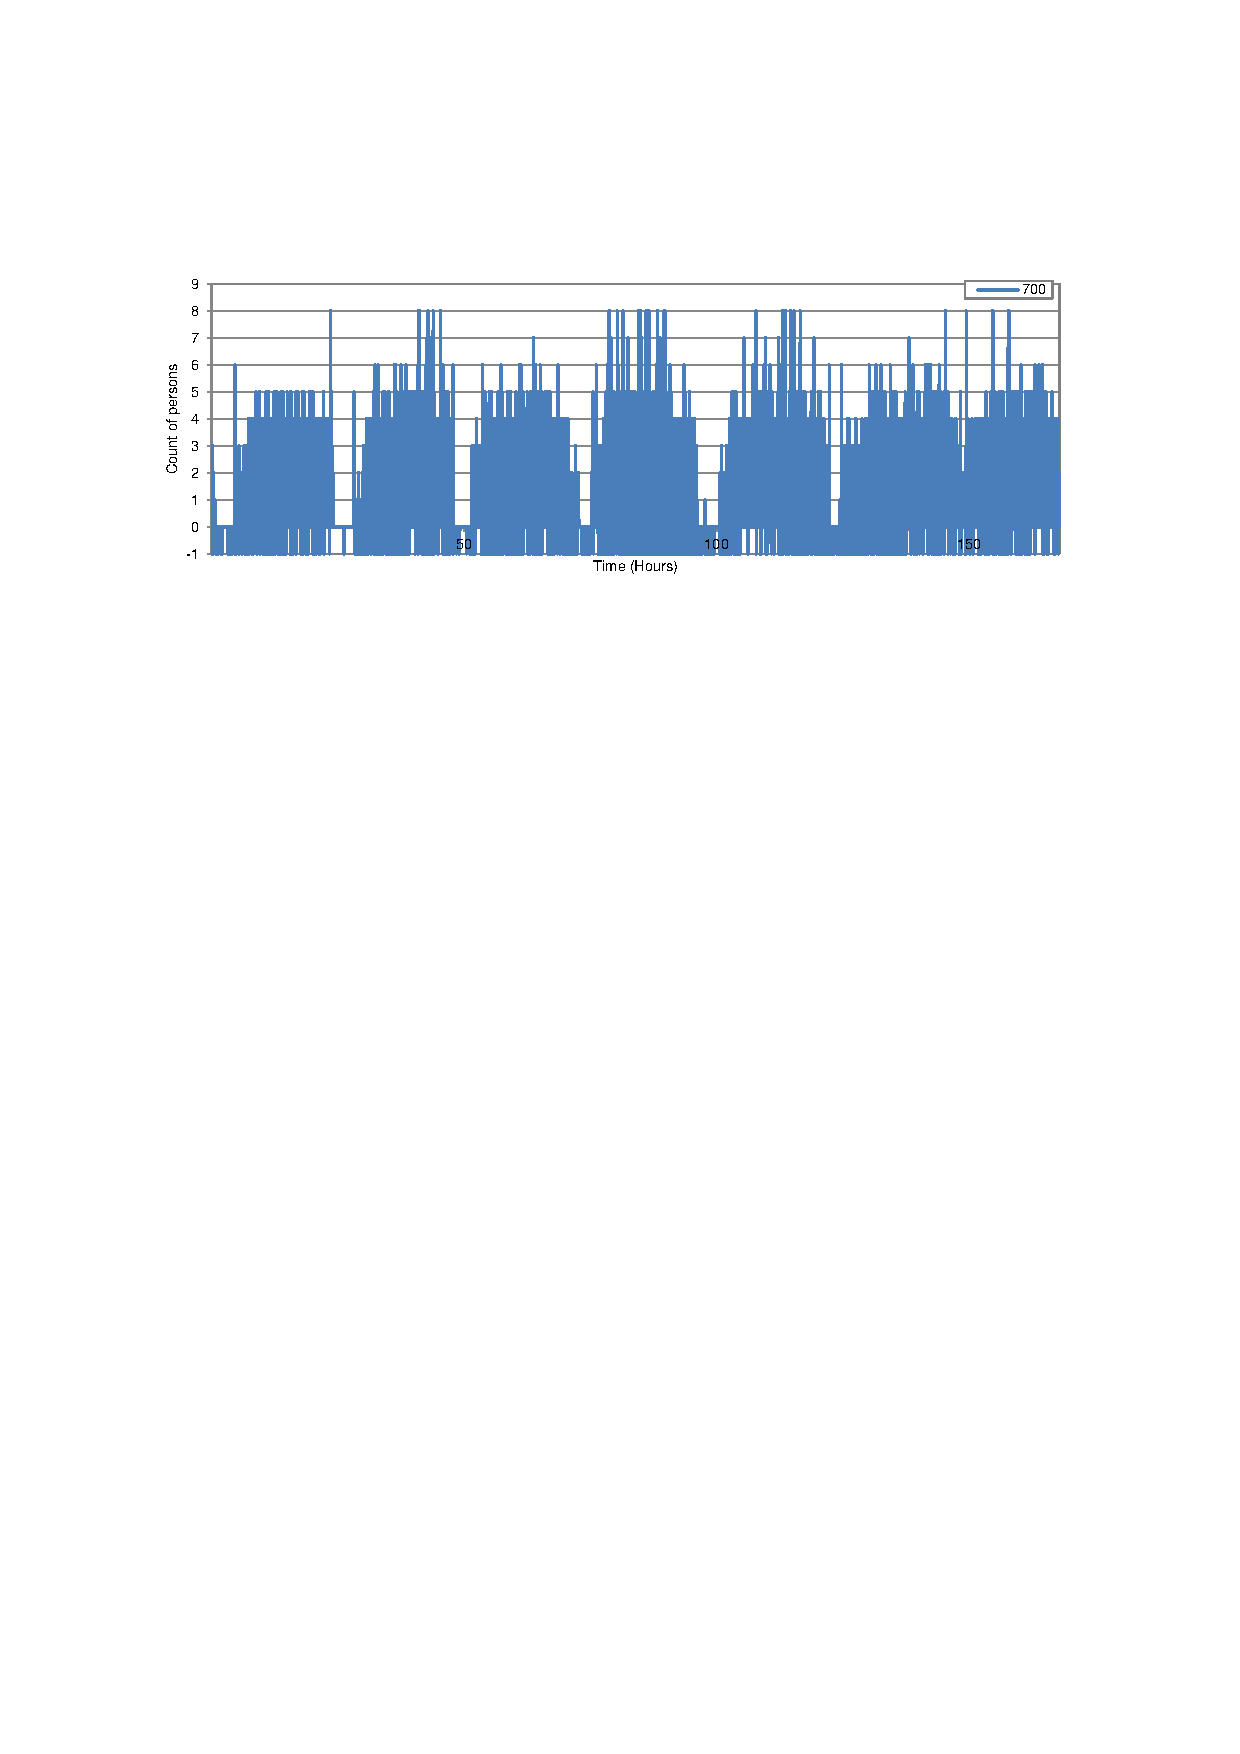
\includegraphics[width=0.46\textwidth]{Figures/rawData_week.pdf}
    \label{fig:rawData_week}
  }
  \hfill
  \subfigure[Passenger density distribution of one camera during one day.] {
    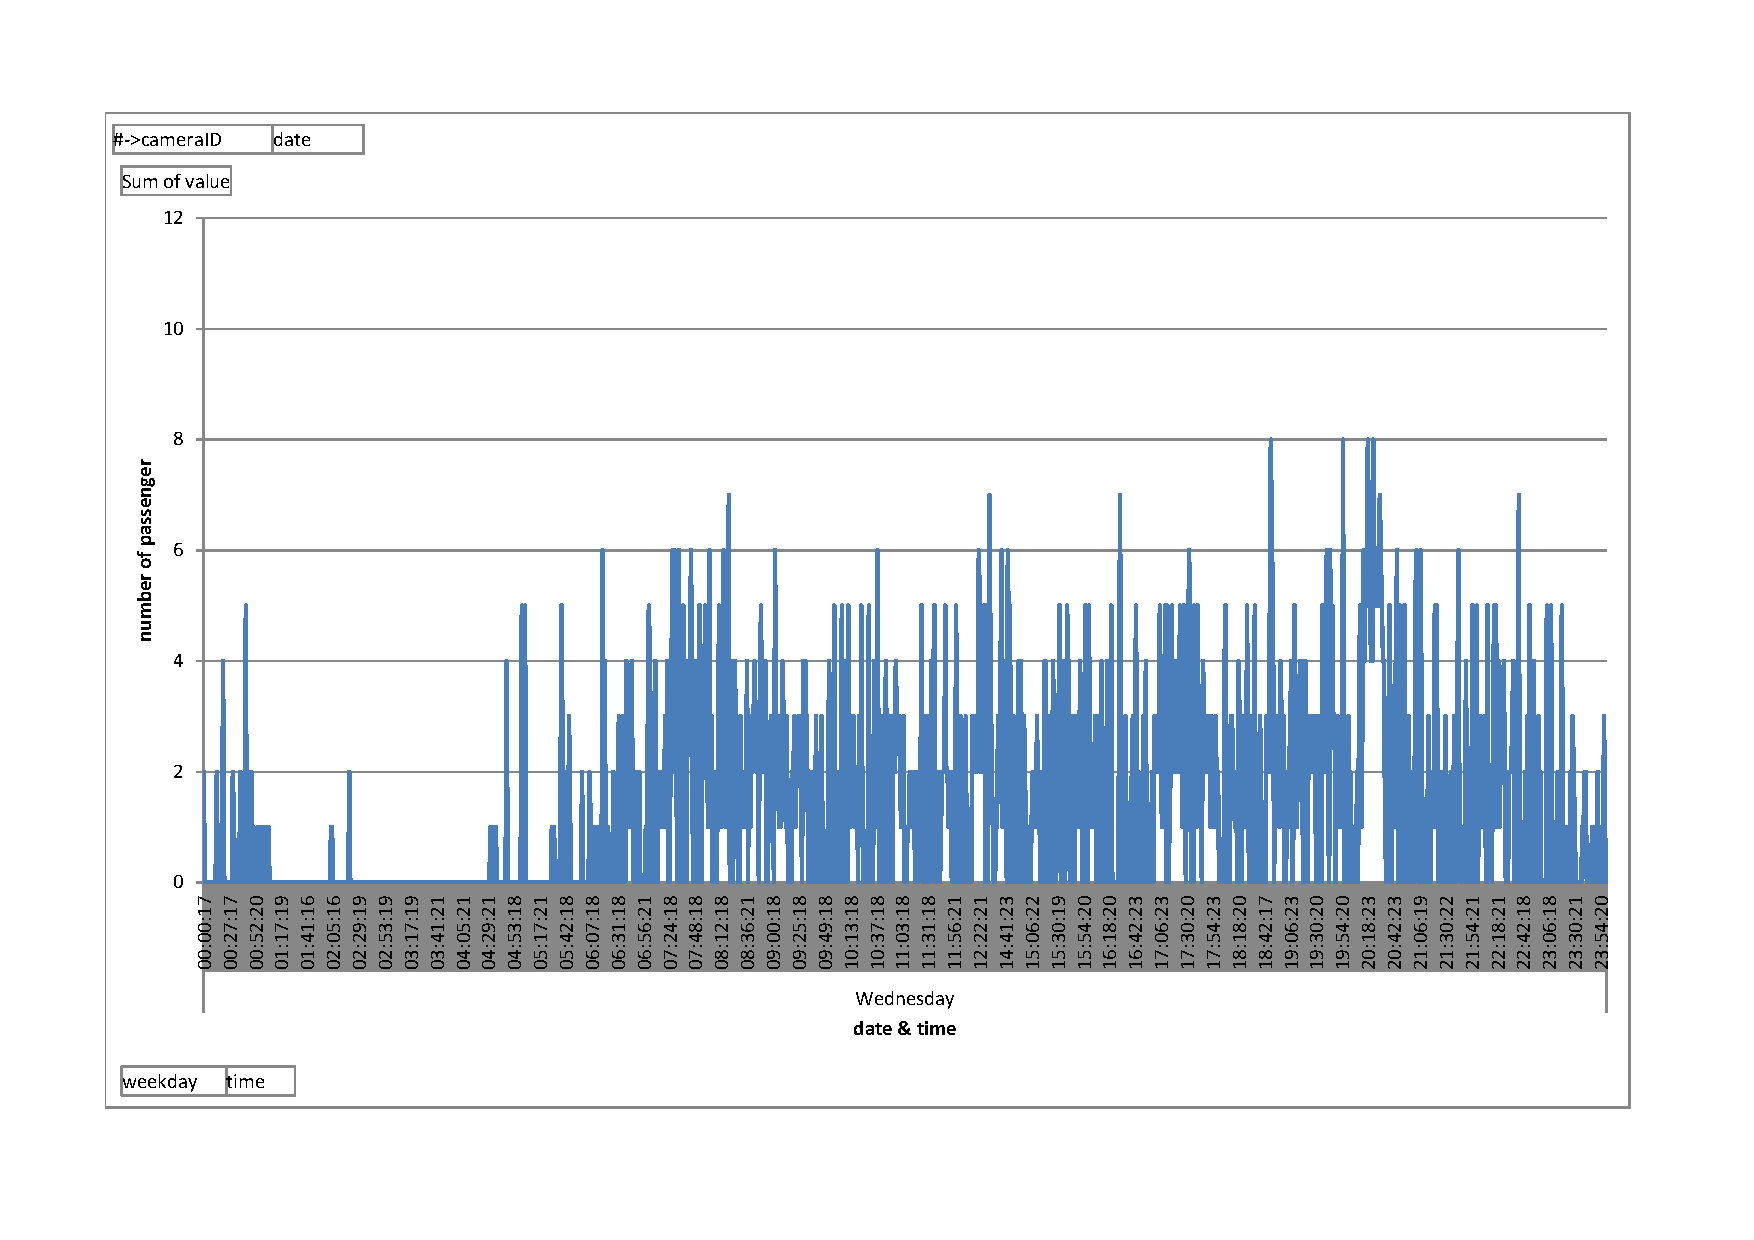
\includegraphics[width=0.46\textwidth]{Figures/rawData_day.pdf}
    \label{fig:rawData_day}
  }

  \caption{Passenger density distribution of one CCTV camera in PdG-L3.}
  \label{fig:rawData}

\end{figure*}

% two columns



% passenger density data
\section{Passenger density data}

\subsection{Properties of the data}
\label{sec:PassengerDensityData}

In order to model the passenger density an understanding of the available data is necessary. In this section the data, visible pattern and other features are discussed.

Figure~\ref{fig:rawData_week} illustrates exemplary the available values of a camera and week. At a more detailed view Figure~\ref{fig:rawData_day} shows the passenger density level of a camera and (week)day. On both Figures, the PdG service times are visible due to the low passenger density level between 01:00 and 05:00 on weekdays.

\begin{figure*}[htbp]

  \centering

  \subfigure[Passenger density distribution of one camera during one week.] {
    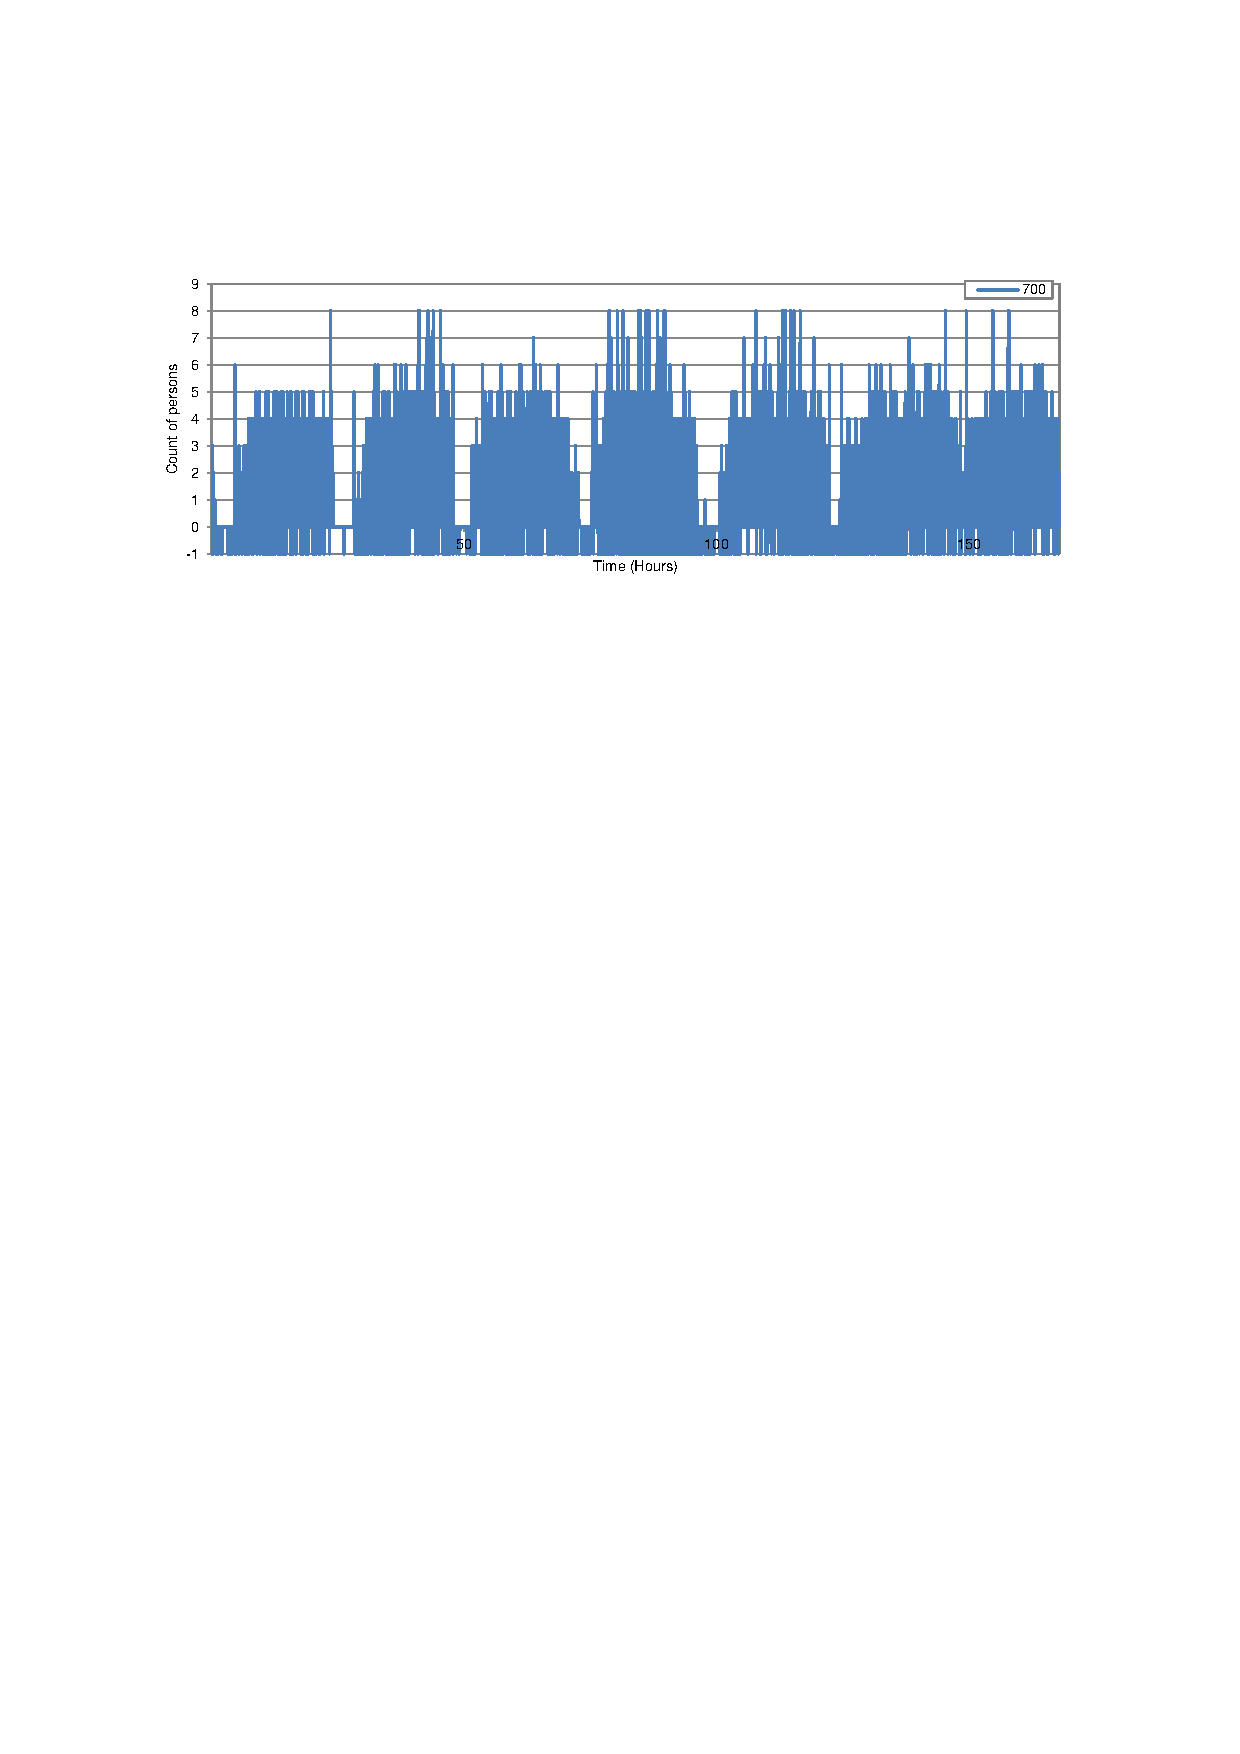
\includegraphics[width=0.46\textwidth]{Figures/rawData_week.pdf}
    \label{fig:rawData_week}
  }
  \hfill
  \subfigure[Passenger density distribution of one camera during one day.] {
    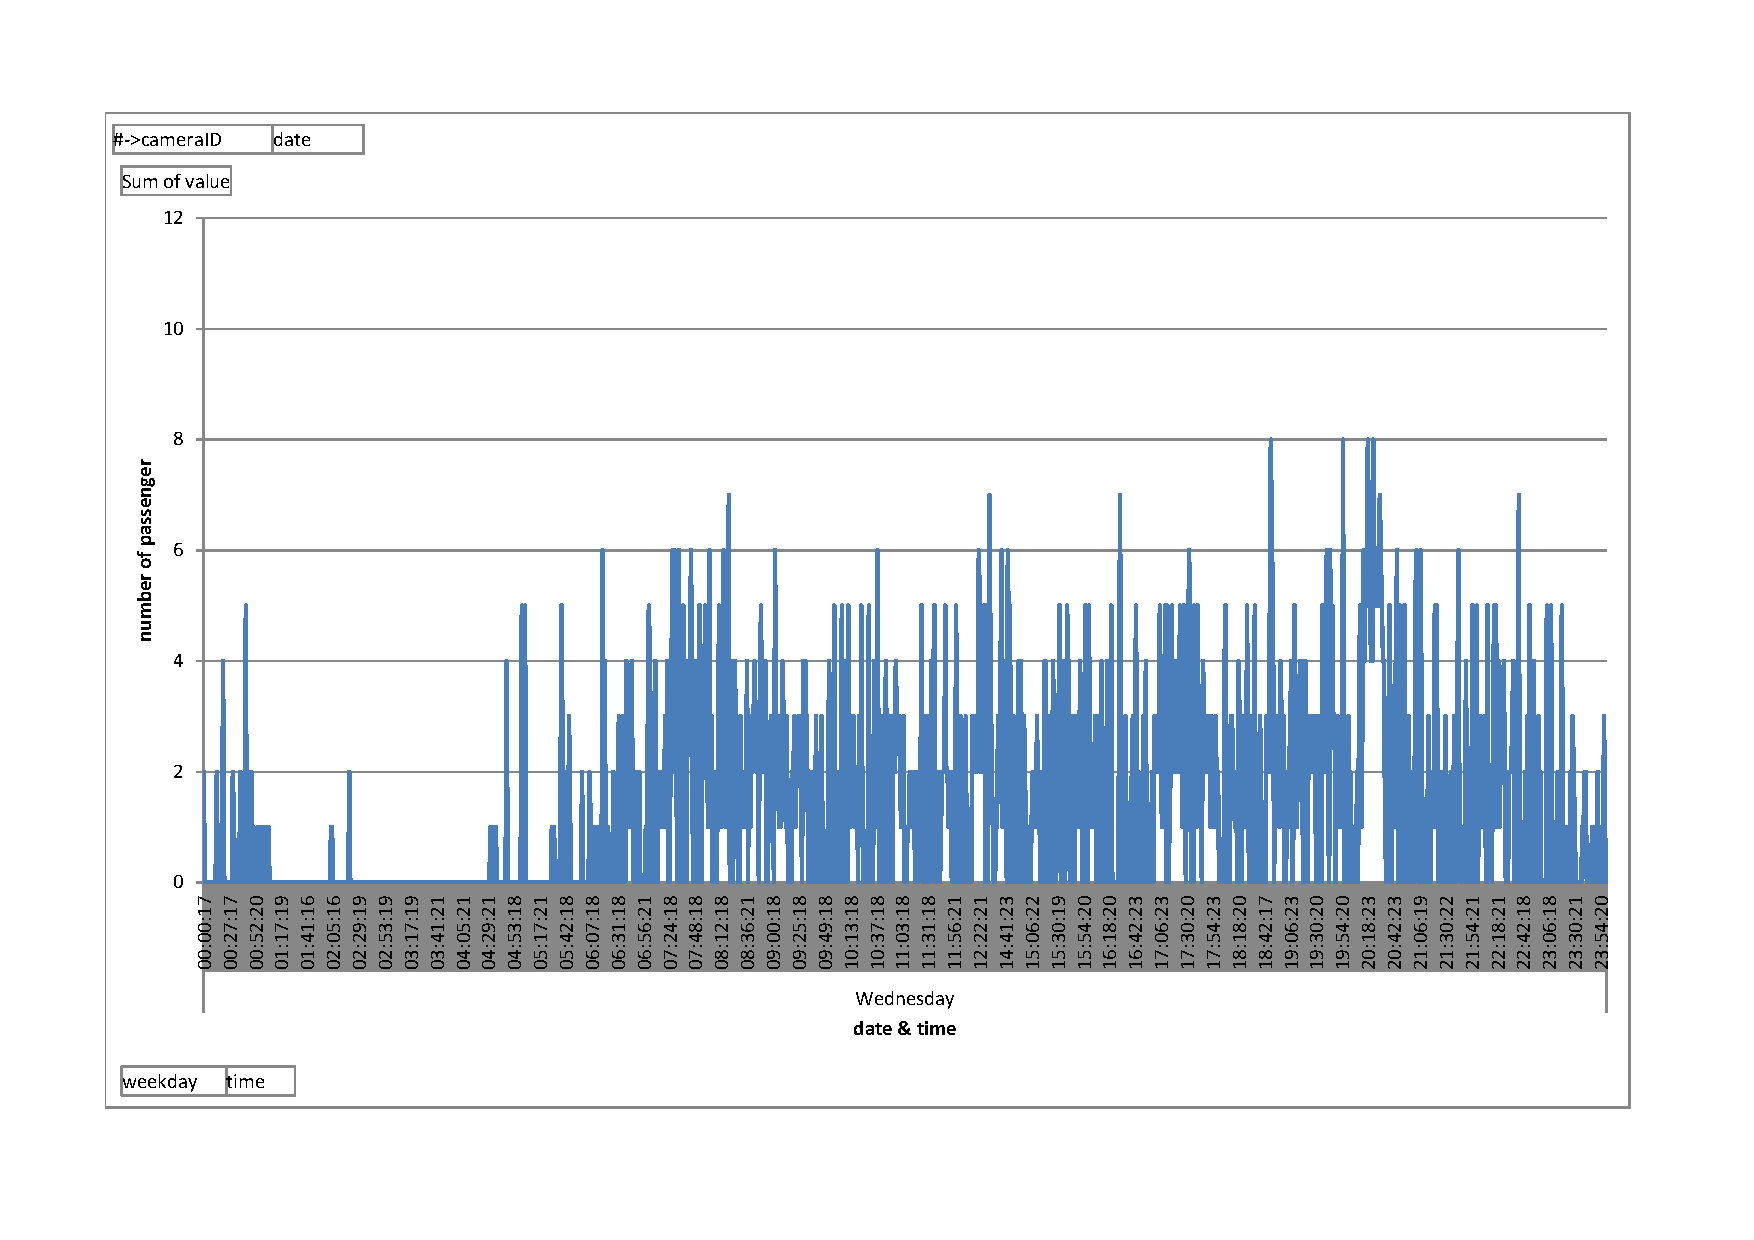
\includegraphics[width=0.46\textwidth]{Figures/rawData_day.pdf}
    \label{fig:rawData_day}
  }

  \caption{Passenger density distribution of one CCTV camera in PdG-L3.}
  \label{fig:rawData}

\end{figure*}


\begin{figure*}
\centering
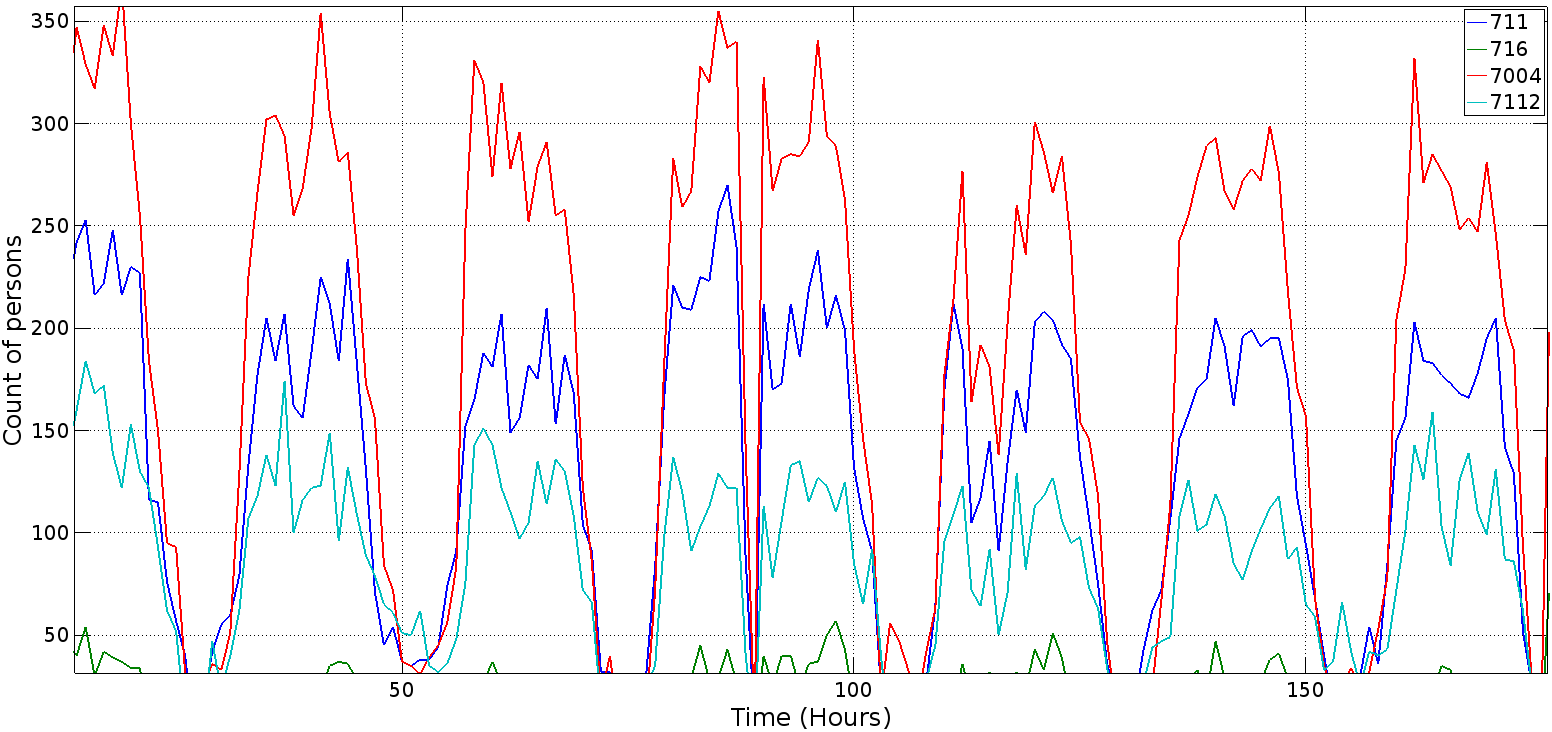
\includegraphics[width=\textwidth]{Figures/Figure_PersonCount_Hours.png}
 \caption{todo}
\end{figure*}

\subsection{Prediction by Artificial Neural Fuzzy Inference System}

\begin{figure*}
\centering
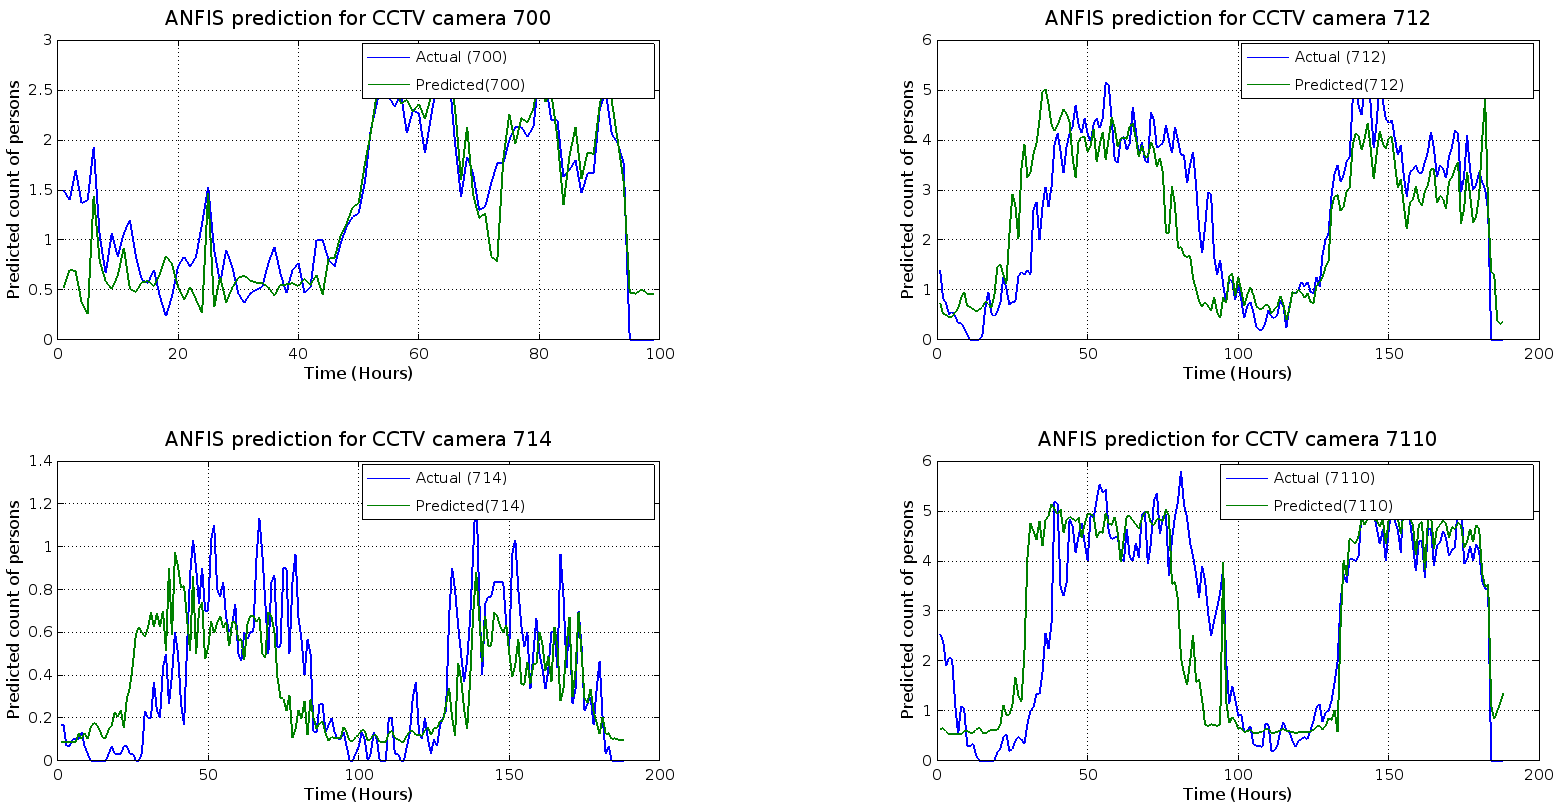
\includegraphics[width=\textwidth]{Figures/Figure_Prediction.png}
 \caption{todo}
\end{figure*}

\begin{figure*}
\centering
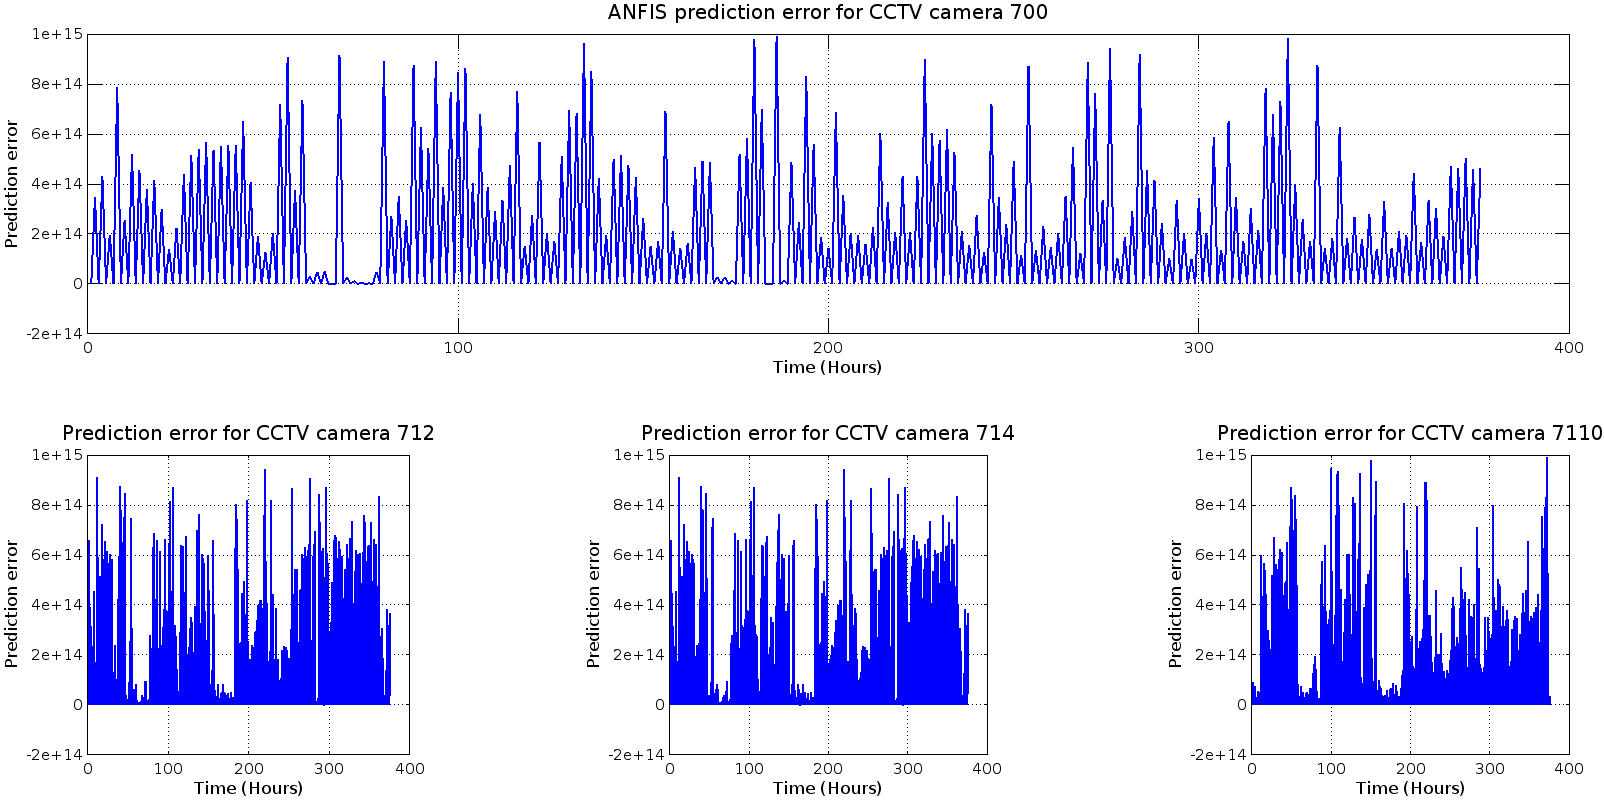
\includegraphics[width=\textwidth]{Figures/Figure_PredictionError.png}
 \caption{todo}
\end{figure*}



% Conlusion
\section{Conclusion}
\label{sec:conclusion}

Conclusion


% Acknowledgemnts
\section{Acknowledgements}
\label{sec:acknowledgements}

This work was partially funded by the EU-FP7 project "Sustainable Energy mAnageMent 4(for) Underground Systems" (SEAM4US, FP7-ICT, EEB-ICT-2011.6.4). The authors would like to acknowledge the contributions of their colleagues.

% \balance

% References
\label{sec:references}
\bibliographystyle{acm-sigchi} %alpha plain
\bibliography{references.bib}


\end{document}